\documentclass[11pt,a4paper]{article}

\usepackage[utf8]{inputenc}
\usepackage[cyr]{aeguill}
\usepackage[francais]{babel}

% Les packages
%\usepackage[french]{babel}
\usepackage{fancybox}
\usepackage{graphics}
\usepackage{color}
\usepackage{latexsym}
\usepackage{amsmath,amsthm,amssymb}
\usepackage[plain]{fullpage} 
\usepackage{verbatim}
\usepackage{times,epsfig}
\usepackage{listings}
\usepackage{multirow}
\usepackage{amsmath,amsthm,amssymb,amscd,txfonts,bbm} % RAJOUT ICI !!!
\usepackage{graphics,epsfig} % RAJOUT ICI !!!
%\usepackage{algorithmic}
\usepackage[final]{pdfpages} 
\usepackage{fancyvrb}
\usepackage{enumerate}
\usepackage{listingsutf8}
\usepackage{comment}
\usepackage{minted}

% small et verbatim: to be coherent with \file
\newenvironment{smallverbatim}%
{\endgraf\small\verbatim}{\endverbatim}

\newenvironment{qv}
{\quote\Verbatim}
{\endquote\endVerbatim}

\usepackage{lastpage}

\newcommand{\terme}[1]{\texttt{#1}}
\newcommand{\termSet}[1]{\{\texttt{#1}\}}
\newcommand{\guill}[1]{<<\,#1\,>>}
% Macro pour l'inclusion de figure  
\newcommand{\fig}[2]{%
  \begin{figure*}[hbt]
   \begin{center}
      \includegraphics[width=6cm]{#1}
  \caption{\label{#1}  #2}
  \end{center}
 \end{figure*}
}
\newcommand{\figTex}[2]{%
  \begin{figure*}[hbt]
 \centerline{\input{#1.pstex_t}}
  \caption{\label{#1}  #2}
 \end{figure*}
}

% Macro commentaires
\definecolor{turquoise}{rgb}{0.20 ,0.60, 0.60}
\definecolor{vert}{rgb}{0.40,  0.60 ,0.00}
\definecolor{violet}{rgb}{0.80 , 0.00 , 0.80}
\definecolor{bleu}{rgb}{0.20,  0.20,  0.80}
\definecolor{rose}{rgb}{1.00,  0.20,  0.40}

\lstset{basicstyle=\footnotesize,showstringspaces=false,language=XML,breaklines=false,columns=fullflexible,frame=shadowbox, captionpos=b}

\newenvironment{solution}[0]{
~\\ \color{red} \textbf{Solution : }\color{black}}{%
}
%\excludecomment{solution}


\newcommand{\cle}[1]{\textbf{#1}}
\def\fk#1{\textit{#1}}
\def\tble#1{\textit{#1}}

\parindent=0pt           
                             
\usepackage{url}

\newtheorem{Exercice}{Definition}


\begin{document}

\title{Sujet d'examen UE NFE204 - Session FOAD}
\author{Année universitaire 2018-2019}
\date{Examen première session: 21 juin 2019}

\maketitle

\begin{center}
{\bf \Large Consignes}\\
\begin{tabular}{| p{15cm} |}
\hline
Dur\'ee de l'examen : 3h00; Documents non autoris\'es;  Calculatrice autoris\'ee\\

Les exercices sont indépendants les uns des autres. Merci de soigner votre écriture.\\
Ce sujet contient \pageref{LastPage} pages.\\

\textit{Important}\,: nous n'évaluons pas les réponses par la syntaxe. Ne vous
inquiétez pas d'utiliser un point-virgule à la place d'un point d'exclamation ou
autres détails mineurs
\\
\hline
\end{tabular}
\end{center}

\emph{L'ensemble de l'examen doit vous permettre de montrer que vous avez assimilé les principales notions vues
en cours et en TP et que vous savez les mettre en application et les expliquer. La clarté, la concision,
la précision des réponses sera donc appréciée.}

\section*{Première partie\,: modélisation par documents structurés (7 pts)}

Le Grand Débat a permis de collecter les contributions de beaucoup de Français. 
Le gouvernement a défini 5 sujets (``Impôts'',
``Transition écologique'', etc.) et proposé un ensemble
de questions pour chaque sujet (ex: ``Payez-vous trop d'impôts'' ou ``Faut-il arrêter d'importer du pétrole'').
Chaque citoyen (anonymisé: on ne connaît que sa région
de résidence) peut alors entrer sa contribution
sous la forme d'un texte libre. 


\begin{figure}[hb]
   \begin{center}
      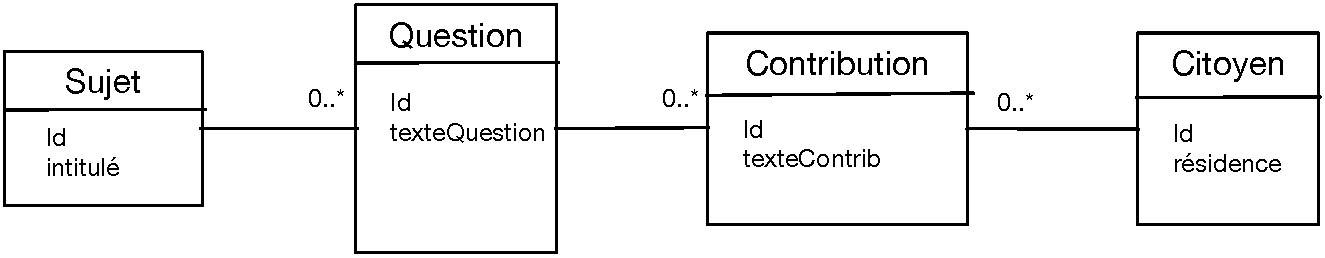
\includegraphics[width=14cm]{schema-granddebat}
  \caption{\label{sgd}  Schéma de la base du Grand Débat}
  \end{center}
\end{figure}

Les contributions sont stockées dans une base relationnelle dont le schéma est donné
par la figure~\ref{sgd} en UML. Elles sont publiées ensuite
sous la forme de documents JSON à des fins d'analyse. 

\begin{enumerate}
  \item Donnez le schéma relationnel correspondant à la figure~\ref{sgd}. 
  \item Donnez un exemple de base relationnelle avec quelques données (très simplifiées) dans chaque table: deux sujets,
      deux questions (une par sujet), trois contributions par deux citoyens. 
      
   \item Donnez une représentation JSON d'un document rassemblant toutes les informations
        (questions, contributions, citoyens) relatives au premier sujet que vous avez choisi.
        
%    \item Donnez une représentation JSON d'un document centré cette fois sur les questions.
    
    \item Indiquez le traitement MapReduce qui permet de passer de la représentation
          précédente à une représentation centrée sur les citoyens.
     
     \item Vous anticipez un très grand nombre de contributions et souhaitez
        donc prévoir un stockage des documents JSON dans un système distribué. Quelle représentation
        vous semble préférable parmi les deux précédentes pour tirer au mieux parti de la distribution\,? 
        
      \item Vous développez un programme \textsc{AnalyseContrib($d$)} qui s'applique à  un
         document $d$ contenant l'ensemble des contributions
          relatives à une question. Quel format ce document devrait-il avoir à
          votre avis pour atteindre une scalabilité maximale\,? 
          Quelle chaîne de traitement permettrait obtenir un tel document
          à partir de l'une des représentations JSON déjà proposées (au choix)\,?
\end{enumerate}

\begin{solution}

\begin{enumerate}
  \item Le schéma de la base
   \begin{enumerate}
       \item Sujet (\textbf{id}, intitulé)
       \item Question (\textbf{id}, texte, idSujet)
       \item Citoyen (\textbf{id}, résidence)
       \item Contribution (\textbf{id}, texteContrib, idCitoyen, idQuestion)
     \end{enumerate}
     
  \item Donnez un exemple de base relationnelle avec quelques données (très simplifiées) dans chaque table: deux sujets,
      deux questions (une par sujet), trois contributions par deux citoyens. 
      
      
\vspace*{0.2cm}
\begin{minipage}[b]{4cm}
\begin{tabular}{l|l}
\cle{id} & nom\\
\hline
20 & Impôts\\
21 & Transition écologique \\
\hline
\end{tabular}

\centerline{La table \tble{Sujet}}
\end{minipage} \hspace*{0.5cm} \
\begin{minipage}[b]{3cm}
\begin{tabular}{l|l|l}
\cle{id} &  nom  & idSujet\\
\hline
100 & Payez-vous trop d'impôts & 20\\
101 & Faut-il arrêter le pétrole & 21\\
\hline
\end{tabular}
\centerline{La table \tble{Question}}
\end{minipage}

\begin{center}

\begin{tabular}{l|c}
\cle{\fk{id}} & Résidence \\
\hline
chocho@monsite.com  & Paris\\
alain@dugenou.com & Marseille\\
\hline
\end{tabular}


\centerline{La table \tble{Citoyen}}

\begin{tabular}{l|c|l|l}
\cle{id} & texteContrib & \fk{idCitoyen} & \fk{idQuestion} \\
\hline
1 & 100 &  chocho@monsite.com& C'est insuportable\\
2  & 100  & alain@dugenou.com & Moi ça me va\\
3 & 101  &  chocho@monsite.com& Surtout pas\\
4 & 101  & alain@dugenou.com & Bien sûr\\
\hline
\end{tabular}

La table \tble{Contribution}
\end{center}
   \item


\begin{minted}[frame=leftline,
               baselinestretch=.9,
               fontsize=\footnotesize,
               framesep=2mm]{json}
{
  "_id": 978,
  "sujet": "Impôts",
  "questions": [
     {
       "question": "Payez-vous trop d'impôts?",
       "contributions": [
          {"citoyen": "chocho@monsite.com",
            "texteContrib": "C'est insuportable"
          },
         {"citoyen": "alain@dugenou.com",
             "texteContrib": "Moi ca me va"
         }
        ]
      },
      {
       "question": "Faut-il arrêter le pétrole",
       "contributions": [
          {"citoyen": "chocho@monsite.com",
            "texteContrib": "Surtout pas"
          },
         {"citoyen": "d@alta.com",
             "texteContrib": "Bien sûr"
             
         }
        ]
      }
    ]
}
\end{minted}        
    
    \item La fonction de Map prend en entrée un document "sujet", effectue une boucle sur les questions
        puis sur les contributions, et émet des paires avec comme clé le citoyen, et comme valeur le sujet, la question
           et le texte de la contribution.
           
           La fonction de reduce agrège toutes les contributions d'un même citoyen en un document JSON.
           
     \item Il n'y a que 5 sujets, ce qui limite les possibilités de distribution. Il faut utiliser les documents 
            centrés sur les citoyens.
        
      \item Un MapReduce produit de documents centrés sur les questions. Même chose que ci-dessus, mais
          avec une boucle en moins dans la fonction de Map.
\end{enumerate}
\end{solution}



\section*{Deuxième partie : recherche d'information (8 pts)}

Maintenant on veut analyser les contributions au grand débat et on commence par
construire un index plein texte. On va travailler sur l'échantillon
suivant des contributions $c_1, ..., c_5$.

% Vin -> impôts
% Plat -> essence
% Décor -> écologie
% Dessert -> logement

\vspace*{0.3cm}

\begin{tabular}{lp{15cm}}
     $c_1$& \texttt{Non seulement on est écrasés d'impôts, mais en plus l'essence augmente sans fin}.\\
     $c_2$& \texttt{C'est bien beau de payer des impôts sur le pétrole ou le logement, il faudrait que ca serve à l'écologie.}\\
     $c_3$& \texttt{Des impôts, encore des impôts. Stop!}\\
     $c_4$& \texttt{Je propose que les taxes sur l'essence financent la rénovation des logements, c'est pour l'écologie.}\\
     $c_5$& \texttt{Acheter de l'essence, c'est payer des impôts. J'en arrive à devoir choisir entre mon essence et mon logement.}\\ 
\end{tabular}

\bigskip

On va se limiter dans un premier temps au vocabulaire (\texttt{impôt, essence, écologie, logement}).
(NB: on suppose
     une phase préalable de normalisation qui élimine les pluriels, majuscules, etc.)

\begin{enumerate}
   \item Donnez une matrice d'incidence (ou index) contenant les tf, 
      et un tableau donnant les idf (sans le $\log$), pour les  termes précédents. Placez
      les termes en ligne, les contributions en colonne.

     Donnez également les normes des vecteurs représentant ces commentaires.
\begin{solution}
\begin{center}
\begin{tabular}{l|c|c|c|c|c}
            & \textbf{c1} & \textbf{c2} & \textbf{c3} &\textbf{c4}&\textbf{c5} \\ \hline  
   impôt  5/4   & 1           & 1           & 2           & 0         & 1\\
   essence 5/3  & 1           & 0           & 0           & 1         & 2\\
   écologie 5/2  & 0           & 1           & 0           & 1         & 0\\
   logement 5/3  & 0           & 1           & 0           & 1         & 1\\\hline
   \end{tabular}
\end{center}

Les normes
\begin{itemize}
  \item $||c_1|| = \sqrt{1+ 1}$; $||c_2|| = \sqrt{3}$; $||c_3|| = \sqrt{4}$; 
    $||c_4|| = \sqrt{3}$, $||c_5|| = \sqrt{6}$  
\end{itemize}
\end{solution}
  
  \item Dans un espace à deux dimensions avec les axes ``impôt'' en abcissse et ``essence'' en ordonnée,
       placer les vecteurs correspondant aux documents normalisés.
       
  \item Donner les résultats classés par similarité cosinus basée sur les tf 
  (on ignore l'idf) pour la requête \texttt{impôt essence}.
    Expliquez brièvement la raison  du classement.

\begin{solution}
Les cosinus (requête non normalisée).

\begin{itemize}
  \item  impôt et essence
  
    c1 : $\frac{1+1}{\sqrt{2}}$; 
    c2 : $\frac{1}{\sqrt{3}}$;
    c3 :  $\frac{2}{\sqrt{3}}$  
    c4 :  $\frac{1}{\sqrt{3}}$  
    c5 : $\frac{1+2}{\sqrt{6}}$; 
 \end{itemize}

\end{solution}  

   \item Quelqu'un remarque que le terme ``taxe'' est synonyme d'``impôt'' et ``pétrole'' d'essence.
      Proposez les changements dans la matrice pour tenir compte de cette synonymie. Qu'est-ce cela
         change pour la requête \texttt{impôt essence}\,? Commentez en particulier
         le classement des documents c1 et c4.
   
\begin{solution}
Un 1 remplace le 0 dans la cellule \texttt{(impôt, c4)}, et l'idf de \texttt{impôt} devient 1 (on pourrait
donc le considérer comme un mot vide).

Le document c4 remonte en seconde position. Il reste derrière c1 qui ne parle \emph{que} d'impôt et d'essence.
\end{solution}   
    
\item Proposez une formule pour mesure la co-occurrence de deux termes, et
     indiquez une méthode pour calculer cet indicateur à partir de la matrice. Quelle
     est la paire de termes ayant la meilleure co-occurrence (en tenant compte des synonymes)\,?


\begin{solution}
Pour chaque paire, on regarde les colonnes qui ne contiennent pas de 0. Les termes \texttt{impôt essence}
ont la meilleure co-occurrence (3 sur 5) en tenant compte des synonymes.
\end{solution}   
    
     \item On considère que le bon résultat d'une recherche avec le terme \texttt{impôt}
             est celui qui tient compte des synonymes, et ramène donc les documents
                contenant soit \texttt{impôt}, soit  \texttt{taxe}. Si on fait une recherche \emph{booléenne}
                (sans classement donc), quel est le rappel
                et la précision pour notre requête \texttt{impôt essence} avant et après l'adaptation de la matrice aux synonymes\,?
\end{enumerate}


\begin{solution}
Avant\,: il manque c4. La précision est 1, le rappel 2/3. Après\,: la précision et le rappel sont à 1. 
\end{solution}   
    
    
\section*{Troisième partie : flux (3 pts)}

Le grand débat ayant lieu en continu, on décide de mettre en place
une chaîne de traitement de flux qui prend en entrée un flux de contributions, nommé
\texttt{fluxContrib}. Voici son code Scala,
très proche de celui vu en cours.


\begin{minted}[frame=leftline,
               baselinestretch=.9,
               fontsize=\footnotesize,
               framesep=2mm]{scala}
 
 case class CompteurMot(mot: String, compteur: Int)
        
 fluxContrib.map({ {str => FiltrageVocabulaire(str, V) }})
            .flatMap ({ str => str.split("\\W+") })
            .map({ m => CompteurMot(m, 1) })
            .keyBy("mot")
            .sum("compteur")
\end{minted}

La fonction \texttt{FiltrageVocabulaire(s, V)} prend une chaîne $s$ en entrée et un vocabulaire $V$,
et renvoie une chaîne $s'$ dans laquelle on ne garde que les mots de $s$ qui appartiennent à $V$.

\begin{enumerate}
 \item Que produit cette chaîne de traitement\,?
 

\begin{solution}
La fréquence des termes
\end{solution}
 
 \item  Y a-t-il un degré de parallélisation maximal lié à l'un des paramètres de ce calcul\,? Lequel
 et pourquoi\,?
 
\begin{solution}
La parallélisation est limitée par la taille du vocabulaire
\end{solution}

 \item  Comment adapter ce traitement pour prendre en compte les synonymes (vous pouvez suppposer
    que vous disposez de toute fonction nécessaire)\,?
 
\begin{solution}
Il faut une structure $S$ contenant les synonymes, et une fonction \texttt{Synonymes(str, S)} qui
remplace tous les mots par le premier synonyme (par exemple). La fonction s'appelle avant le 
\texttt{flatMap}.
\end{solution}
\end{enumerate}

\section*{Quatrième partie : question de cours (2 pts)}

Dans un système de stockage distribué de type Master-Esclave, vaut-il mieux lire en passant par
    le maître ou en allant directement sur l'esclave qui stocke le document cherché\,? Discuter
      des avantages et inconvénients des deux solutions.

\end{document}
